% \renewcommand{\thefigure}{A.\arabic{section}.\arabic{figure}hhh}
\counterwithin{figure}{section}
\setcounter{section}{2} % Assuming section A.2 corresponds to section 2
\setcounter{figure}{0}  % Reset figure counter for this section
\label{Navigation_SupplementaryInformation}


%%%%%%%%%%%%%%%%%%%%
%% SUPPLEMENTARY %%%
%%%%%%%%%%%%%%%%%%%%


\begin{figure}[htbp]
  \centering
  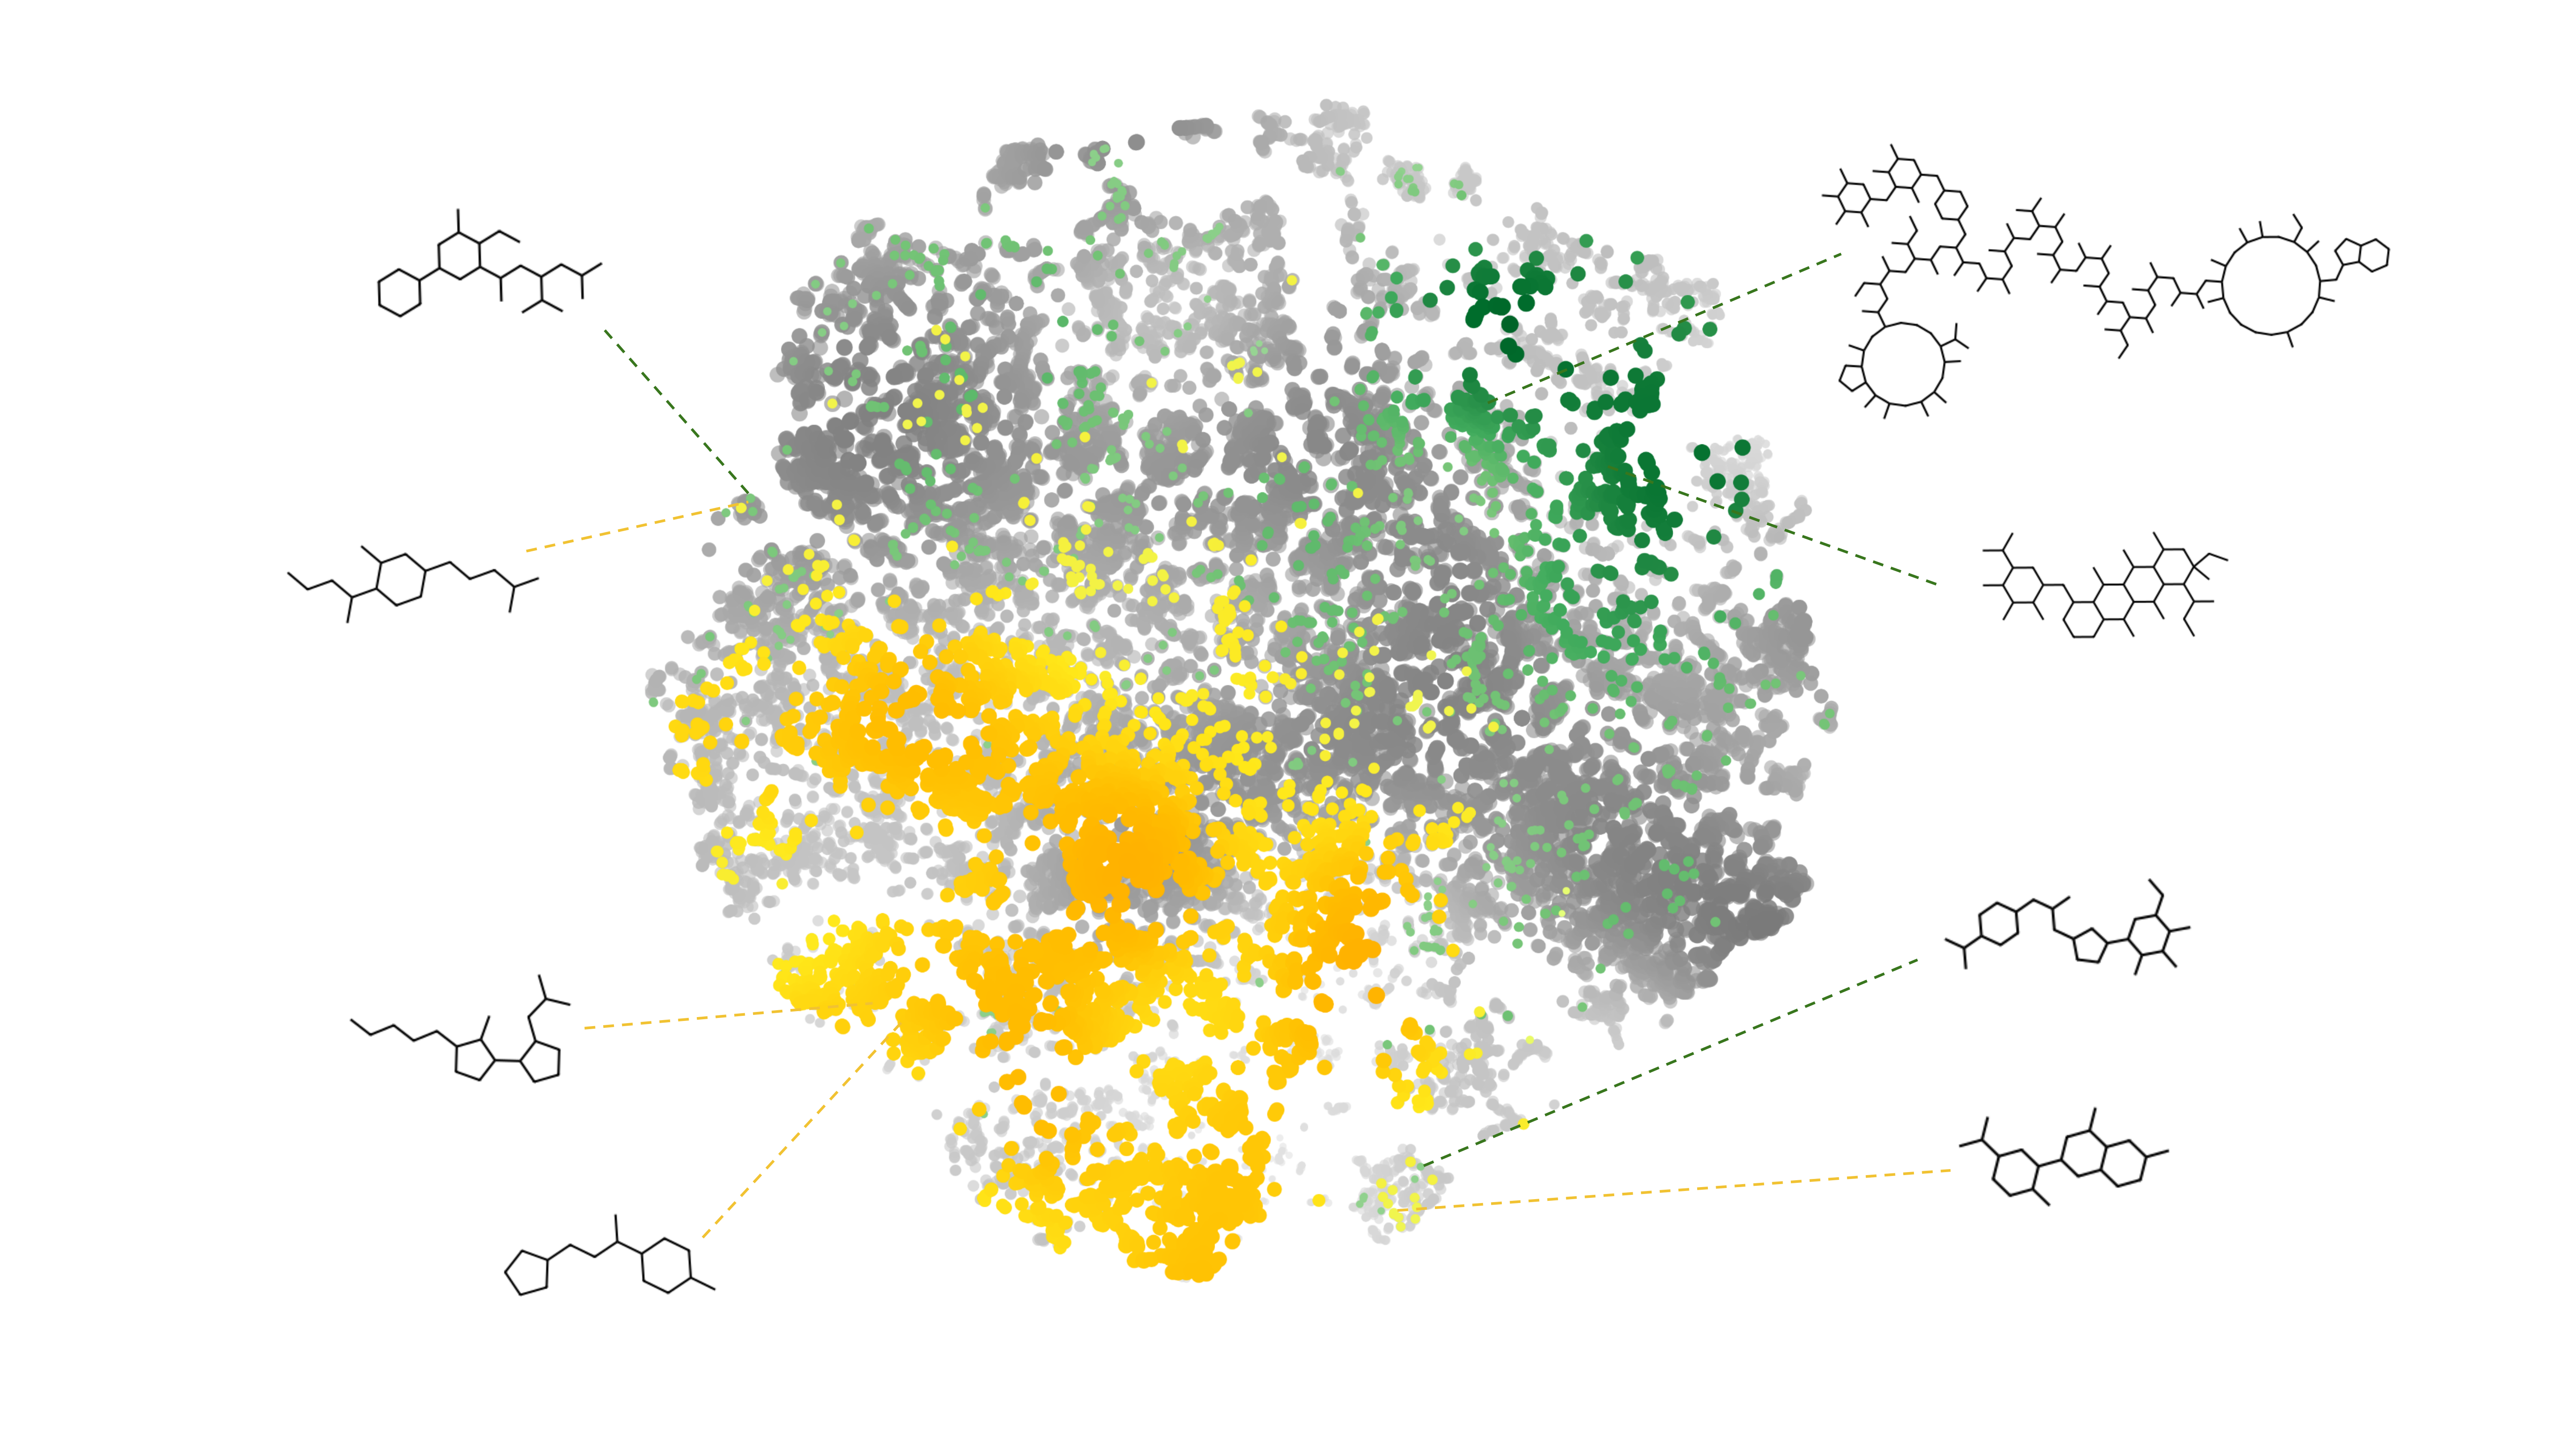
\includegraphics[width=1\linewidth]{figures/Navigation/Supplementary/Medina_v.2.png}
  \caption{2D tSNE representation of the 31,052 selected molecules based on the combined A1-A3-A4 CC signatures (the three spaces are concatenated to obtain 384-length signatures, i.e. 3x128). Green points correspond to Medina’s natural products; yellow points represent 5,000 compounds from the proprietary IRB library. Example molecule scaffolds are displayed for both libraries.
  }
  \label{Navigation_FigS1}
\end{figure}


\begin{figure}[htbp]
  \centering
  \includegraphics[width=1\linewidth]{figures/Navigation/Supplementary/filter.png}
  \caption{Physicochemical properties of the 1,521,567 compounds included in the ChemDiv library: presence of PAINS, molecular weight (MW), topological polar surface area (tPSA), alogP, number of hydrogen bond acceptors, number of hydrogen bond donors, number of rotatable bonds, number of aromatic rings and presence in other libraries (the previous version of the IRB Library, the RNA library, the Covalent library and the Fragments library). Green bins indicate compounds that met the established criteria; red bins indicate those that fell outside the criteria.
  }
  \label{Navigation_FigS2}
\end{figure}


\begin{figure}[htbp]
  \centering
  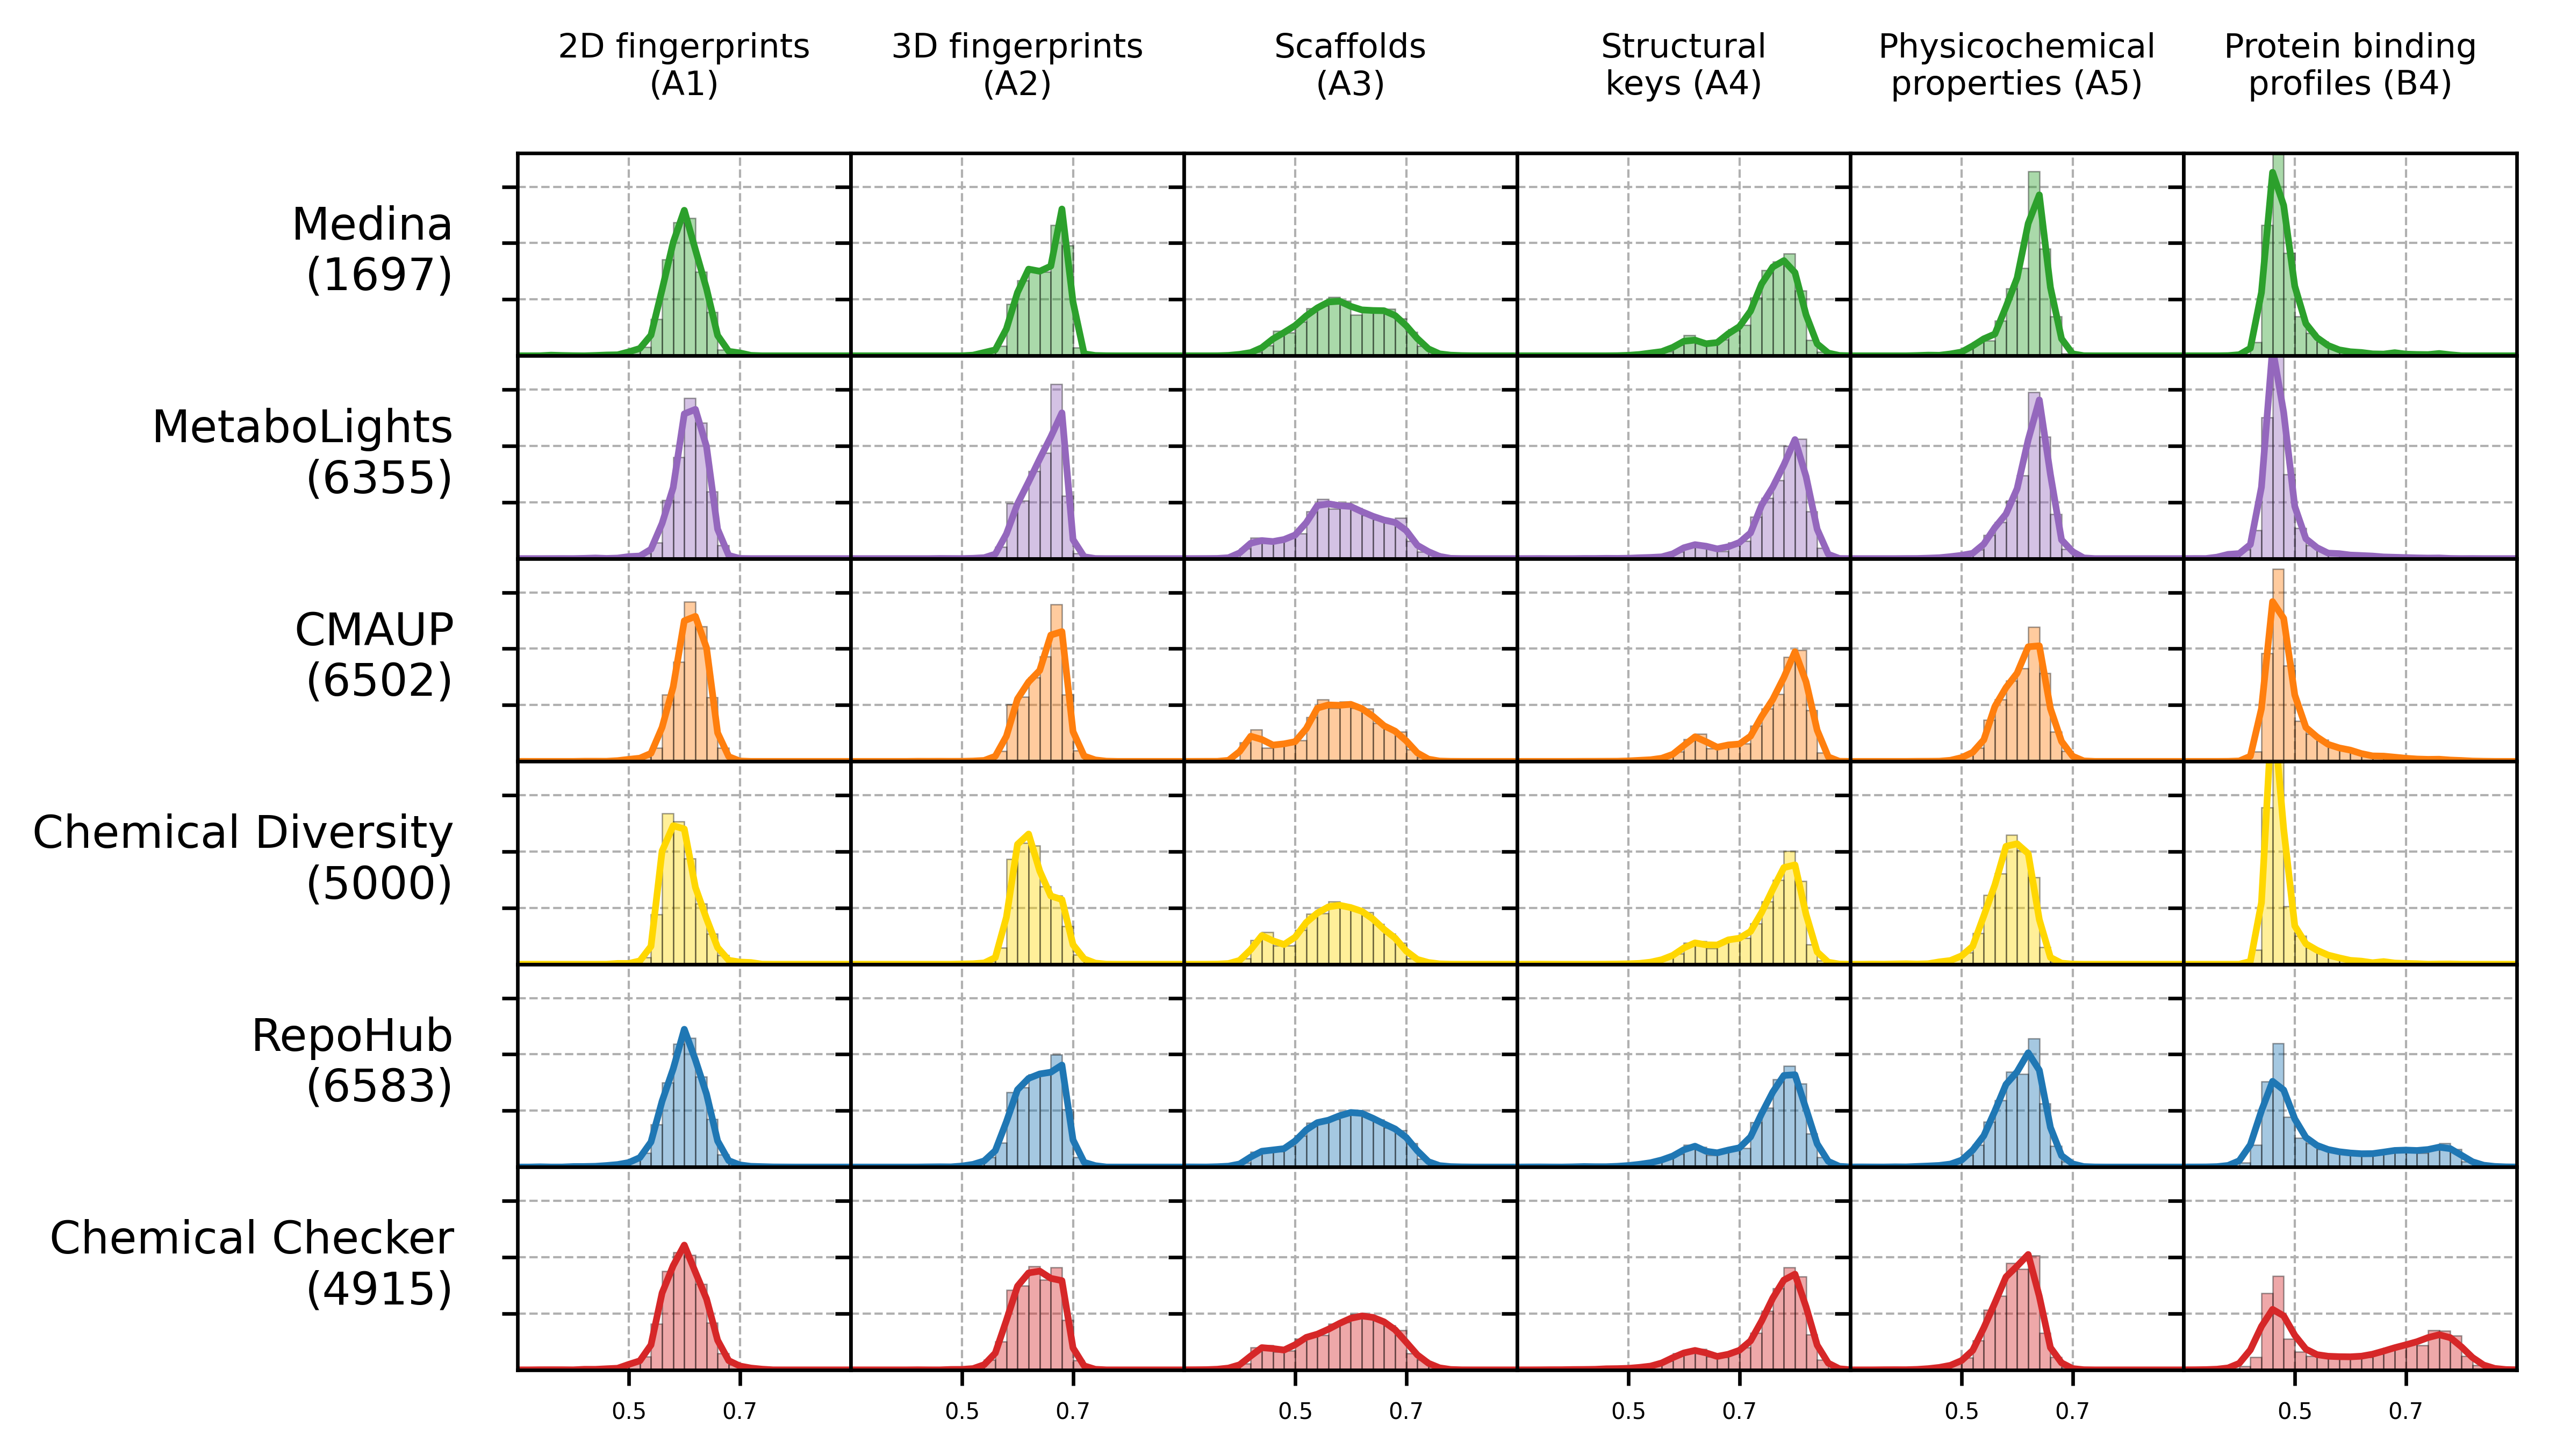
\includegraphics[width=1\linewidth]{figures/Navigation/Supplementary/applicability.png}
  \caption{Distribution of applicability values for the generated CC signatures (A1-A5 and B4 CC spaces) for the 6 selected compound libraries (Medina, MetaboLights, CMAUP, Chemical Diversity, RepoHub and the Chemical Checker).
  }
  \label{Navigation_FigS3}
\end{figure}


%%% ADD TEXT HERE


